Fundamentally, the existence of non--zero temperature--dependent volume expansion coefficients for solids arise from the fact that atomic vibrations are not strictly harmonic. The anharmonic nature of the lattice vibration is often reflected in the change of the vibrational frequencies with respect to the cell volume, a quantity that is captured by the mode--dependent Gr\"{u}neisen parameter,\cite{dolling1966thermodynamic} defined as:
\begin{equation}\label{eq:gruneisen}
    \gamma_{\bm{q},n}=-\frac{\partial \ln \omega_{\bm{q},n}}{\partial \ln V}.
\end{equation}
It can be shown that the lattice expansion coefficient $\alpha=(\partial V/\partial T)_p$ can be derived from the change in the Helmholtz free energy [\cref{eq:helmholtz}] with respect to volume, which can only be non--zero if some phonon modes of the material possess  non--zero $\gamma_{\bm{q},n}$. 

Returning back to the real space view of atomic vibrations, the vibrational anharmonicity arises when the PES $E(\bm{R})$ traced by an vibrating atom in the solid, particularly at large vibrational amplitudes, can only be satisfactorily described by taking the  Taylor expansion of $E(\bm{R})$ that involves the contributions from higher--order force--constants:
\begin{align}\label{eq:higher_order_vib_Hamiltonian}
E(\bm{R})=&\mathcal{U}(\bm{R}_{0})+\bm{\Phi}_{i}^{\alpha}\Delta\bm{R}_{i}^{\alpha}+\frac{1}{2!}\bm{\Phi}_{ij}^{\alpha\beta}\Delta\bm{R}_{i}^{\alpha}\Delta\bm{R}_{j}^{\beta}\nonumber \\&+\frac{1}{3!}\bm{\Phi}_{ijk}^{\alpha\beta\gamma}\Delta\bm{R}_{i}^{\alpha}\Delta\bm{R}_{j}^{\beta}\Delta\bm{R}_{k}^{\gamma}+\frac{1}{4!}\bm{\Phi}_{ijkl}^{\alpha\beta\gamma\delta}\Delta\bm{R}_{i}^{\alpha}\Delta\bm{R}_{j}^{\beta}\bm{R}_{k}^{\gamma}\Delta\bm{R}_{l}^{\delta}+\mathcal{O}(\Delta\bm{R}^{5}),
\end{align}
meaning the topology of $E(\bm{R})$ deviates significantly from a parabolic shape. In highly anharmonic materials, such as cubic perovskites \ce{SrTiO3}, significant contributions to the above expansion can even be found from the sixth order force constant.\cite{tadano2015self} This also implies that, in practical computation of anharmonic lattice dynamics of materials, one should use an energy model, such as DFT [\cref{sec:DFT}], rather that empirical atom-atom potentials [\cref{sect:empirical_forcefield}] that typically truncate the above series at the second order, as it is usually easier to parameterise.

\paragraph{\textbf{Weakly anharmonic systems}} For systems with weak vibrational anharmonicity, the expansion beyond the third order in \cref{eq:higher_order_vib_Hamiltonian} can be satisfactorily disregarded. Extending the finite--displacement method for calculating the harmonic force constant [\cref{eq:FC_finite_difference}], the third order force constant can be calculated as:
\begin{equation}\label{eq:FC3_finite_difference}
    \bm{\Phi}_{ijk}^{\alpha\beta\gamma}\approx-\frac{\bm{F}_{i}^{\alpha}(\Delta\bm{R}_{j}^{\beta},\Delta\bm{R}_{k}^{\gamma})-\bm{F}_{i}^{\alpha}(\Delta\bm{R}_{j}^{\beta})}{\Delta\bm{R}_{j}^{\beta}\Delta\bm{R}_{k}^{\gamma}}. 
\end{equation}
Calculating $\bm{\Phi}_{ijk}^{\alpha\beta\gamma}$ via this approach is in principle only feasible for crystals with small unit cell and high symmetry. This is because \cref{eq:FC3_finite_difference} involves the force contributed by displacing a combination of two atoms along two different Cartesian directions, and the total number of unique combinations in a crystal structure grows factorially as the total number of atoms per cell increases and the crystal symmetry reduces. Although in rare cases, it has been applied in the investigations of selected complex materials, such as hybrid halide perovskites.\cite{zhu2019mixed}

Taking the Fourier transform of $\bm{\Phi}_{ijk}^{\alpha\beta\gamma}$ leads to third--order force constant $\bm{\Phi}_{\lambda\lambda^{\prime}\lambda^{\prime\prime}}$ in the reciprocal space, which contains the information on the strength of interactions among three phonons,\cite{phono3py} and $\lambda=(\bm{q},n)$ is an abbreviation for a specific phonon mode. It means the lowest order contribution to the anharmonic lattice vibration comes from the three--phonon scattering process,\cite{pathak1965theory} which further leads to the finite lattice thermal conductivity ($\kappa_L$) in solids. Otherwise, $\kappa_L$ becomes infinite if the lattice vibration is strictly harmonic in a defect--free crystal.\cite{allen1993thermal} Furthermore, since the crystal is weakly anharmonic, the three--phonon scatterings can be treated perturbatively as a correction to the harmonic phonon, which gives rise to the phonon self--energy $\Sigma_\lambda (\omega_\lambda)$. The imaginary part of $\Sigma_\lambda (\omega_\lambda)$, dubbed as $\Gamma_{\lambda}(\omega_\lambda)$,  represents the finite width  of phonon peak at $\omega_\lambda$, which is proportional to $|\bm{\Phi}_{\lambda\lambda^{\prime}\lambda^{\prime\prime}}|^2$ and can be determined based on the Fermi Golden rule.\cite{maradudin1962scattering} Consequently, this results in the finite lifetime for a given phonon mode $\tau_\lambda=[2\Gamma_{\lambda}(\omega_\lambda)]^{-1}$ according to the Heisenberg's uncertainty principle. This reciprocal relationship means that a phonon mode that is strongly scattered by the others will have a particularly short lifetime. Together with the phonon group velocity $\bm{v}_{\lambda}=\partial \omega_\lambda/\partial \bm{q}$, the lattice thermal conductivity tensor may be obtained by solving the linearised phonon Boltzmann equation under the relaxation time approximation as:\cite{chaput2013direct}
\begin{equation}\label{eq:ph_boltzmann}
    \bm{\kappa}_{L} = \frac{1}{NV}\sum_\lambda C_\lambda \bm{v}_{\lambda}\otimes \bm{v}_{\lambda} \tau_\lambda,
\end{equation}
in which $C_\lambda$ is the mode contribution to the heat capacity [\emph{c.f.} \cref{eq:Cv}]. The above discussion highlights the most commonly adopted approach for computationally determining the lattice thermal conductivities for weakly anharmonic materials.\cite{phono3py,li2014shengbte}  

\paragraph{\textbf{Quantifying the degree of vibrational anharmonicity}} 

Given that the phonon life time $\tau_\lambda$ in \cref{eq:ph_boltzmann} is determined by treating the three--phonon interactions perturbatively, a nature question to ask is how the degree of vibrational anharmonicity can be quantified in order to facilitate the choice of appropriate theoretical approach to model and understand both the structural dynamics and thermal properties of functional materials.  

Theoretically, AIMD simulation is capable to provide us with a set of atomic displacements and forces $\{\Delta\bm{R},\bm{F}\}$, that is governed by  the structural dynamics of a given material in which  all degrees of anharmonicity are accounted for [\cref{eq:higher_order_vib_Hamiltonian}]. If the corresponding harmonic force constant $\bm{\Phi}_{ij}^{\alpha\beta}$ is also known, the corresponding \emph{harmonic force} $\bm{F}^{(2)}$ at any given $\Delta\bm{R}$ can also be determined based on \cref{eq:harmonic_forces}, whereby the difference $\bm{F}^{A}=\bm{F}-\bm{F}^{(2)}$ is naturally the remainder of the atomic force that is contributed by the force--constants beyond the harmonic terms. Based on this fundamental understanding, \citet{knoop2020anharmonicity} proposed an \emph{anharmonic score} to access the degree of vibrational anharmonicity by comparing the standard deviations in $\bm{F}^{A}$ and $\bm{F}$ as sampled from AIMD simulations:
\begin{equation}\label{eq:anharmonic_score}
    \sigma^{(2)}(T)=\sqrt{\sum_{i,\alpha}\left\langle \left(F^{\alpha,A}_{i}\right)^2 \right\rangle_{T}\Big/ \sum_{i,\alpha}\left\langle \left(F_{i}^{\alpha}\right)^2 \right\rangle_{T}},
\end{equation} 
where the summation is performed over the  atoms ($i$) in the simulation cell and the Cartesian direction ($\alpha$). Generally, systems with $\sigma^{(2)}<0.5$ are considered to be weakly anharmonic in which the expansion \cref{eq:higher_order_vib_Hamiltonian} can be safely truncated at the third--order term, whereas those with $\sigma^{(2)}>1$ are structurally not stable at a given $T$. This  criteria is supported by the results obtained from screening the room--temperature stabilities across a large set of 3819 cubic perovskite.\cite{yang2021altas}

\paragraph{\textbf{Strongly anharmonic systems}} 

\begin{figure*}[tb]
    \centering
    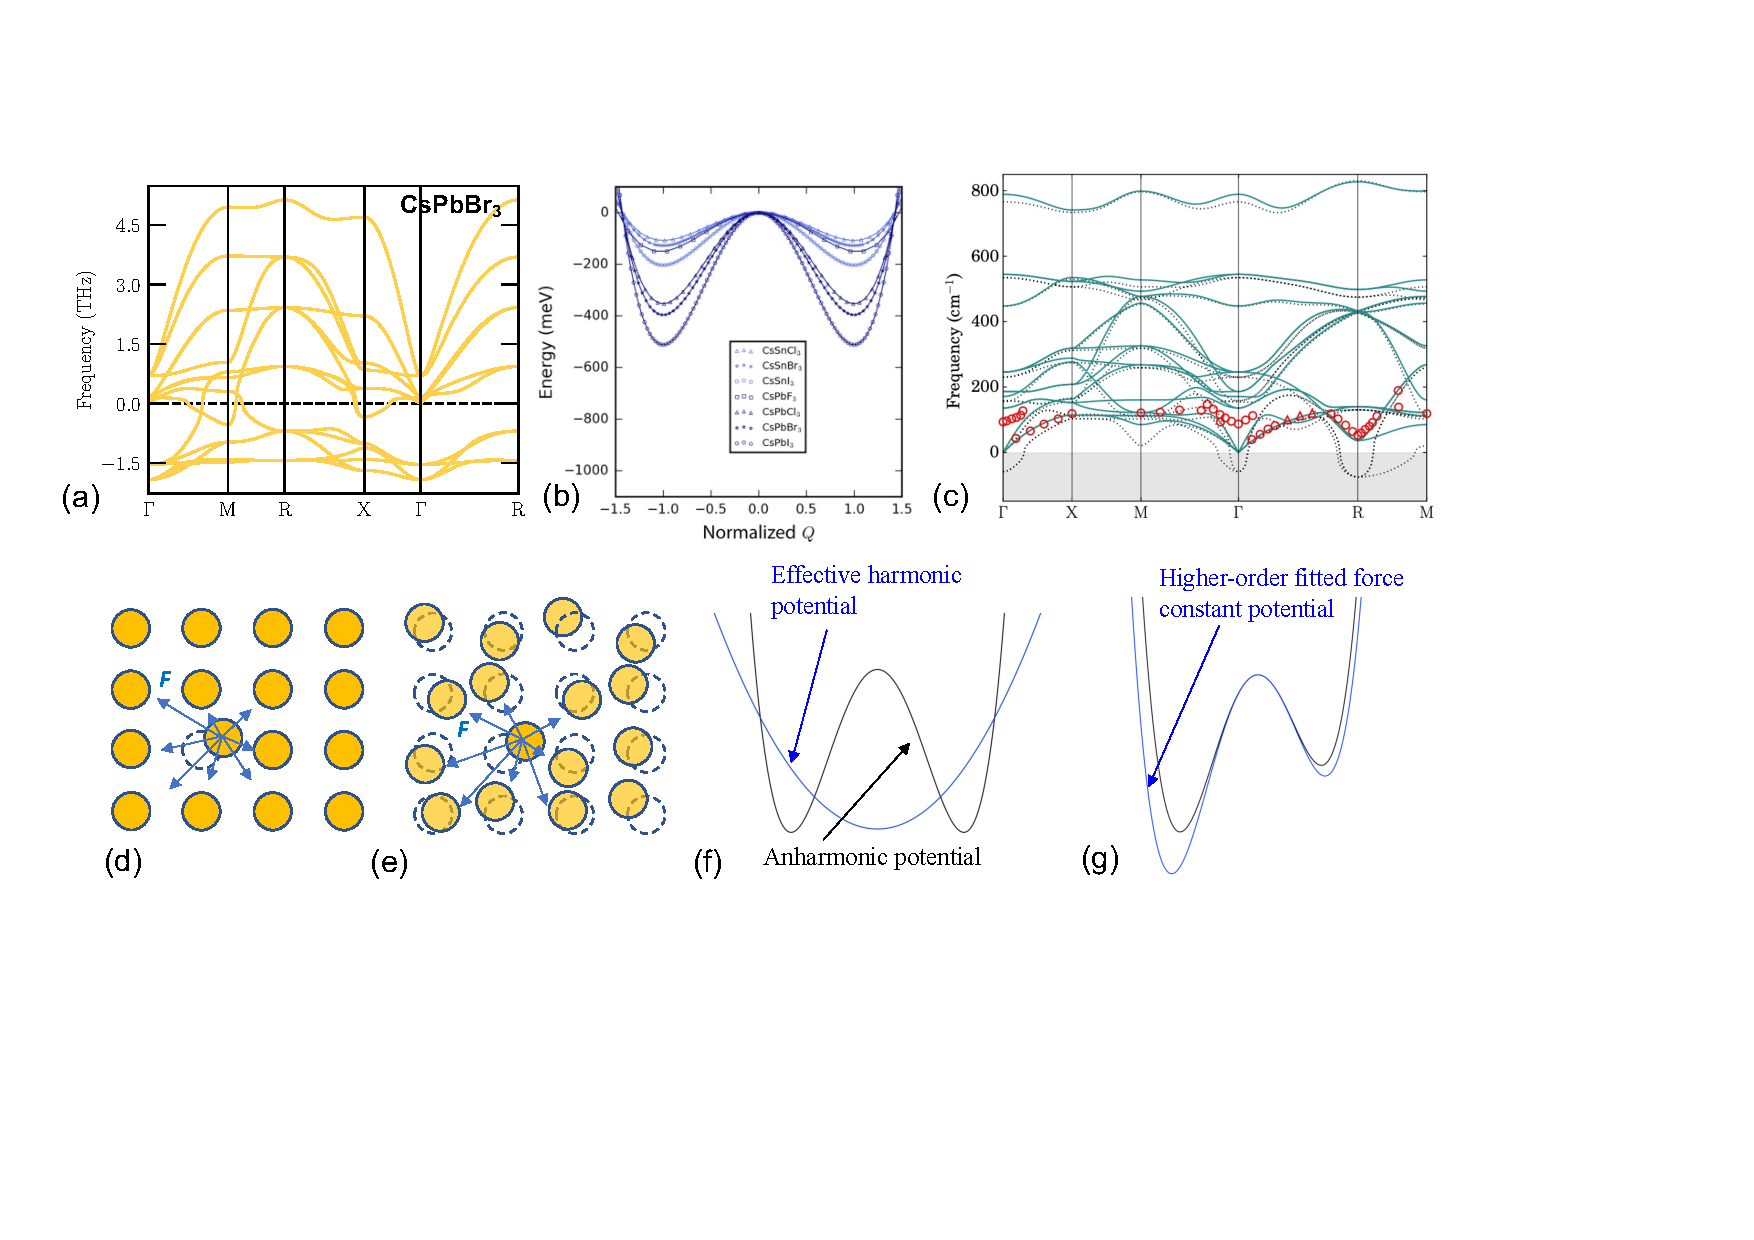
\includegraphics[width=\textwidth]{anharmonic_phonon_illustration.pdf}
    \caption{Strongly anharmonic phonons in cubic perovskites. (a) Phonon dispersion relationship for cubic \ce{CsPbBr3}\cite{yang2021altas} showing the presence of imaginary phonon modes in the system. (b) Double--well potential energy surface of phonon instabilities  in various cubic cesium halide perovskites. The potential energy surface is plotted against the normalised atomic displacements along the normal mode $\bm{\mathcal{Q}}$ that corresponds to the $M_3^{+}$ octahedral tilting.\cite{yang2020assessment}  (c) Comparison of the anharmonic renormalised (solid line) and harmonic (dashed line) phonon dispersion relationship for cubic \ce{SrTiO3},\cite{tadano2015self} showing the dynamic stabilisation of \ce{SrTiO3} at 300 K with the disappearance of the imaginary modes, which is consistent with the experimental results.\cite{cowley1969relationship,stirling1972neutron} (d--e) Schematic illustration of the difference between phonon calculations performed with frozen phonon (d) and  temperature--dependent effective potential (TDEP)\cite{hellman2011lattice,hellman2013temperature} (e). In the frozen phonon approach, the force on a displaced atom is evaluated in an environment of its stationary neighbours, whereas in TDEP, the same force is evaluated in neighbouring atoms that are also moving under thermal excitation. (f) In the original TDEP formalism, an anharmonic double--well--type potential is refitted to an effective harmonic potential. (g) Extension of the TDEP concept to extract higher--order force constants enabling the reconstruction of the anharmonic potential energy surface.\cite{eriksson2019hiphive}}
    \label{fig:anharmonic_phonon_illustration}
\end{figure*}

Materials that possess imaginary phonon frequencies ($\omega_{\bm{q},n}^2<0$) are generally considered to be highly anharmonic, which is also referred to as the phonon instability. This is widely observed in material systems, such as the high--symmetry cubic ABX$_{3}$ perovskites [\cref{fig:anharmonic_phonon_illustration}(a)]. Geometrically, it implies that a given structure is located on a local maximum of the PES with negative curvature, rather than a minimum. Hence, according to \cref{eq:PES_normal_mode_displaced},  the atomic vibrations along the imaginary phonon mode provides additional energetic contributions to stabilise the system. For example, the octahedral tiltings [\cref{fig:anharmonic_phonon_illustration}(b)] in cubic perovskites stabilize the structure by minimising the effect of ionic size mismatches for the constituent ions in adopting a perfect cubic crystal structure in the space group of $Pm\bar{3}m$.\cite{aschauer2014competition} This also implies that, in the higher--order expansion of the PES [\cref{eq:higher_order_vib_Hamiltonian}],   it is critical to include the quartic order term in order to correctly model the lattice dynamics of perovskites that are strongly affected by the double--well potentials, such as the ones shown in  \cref{fig:anharmonic_phonon_illustration}(b). However, as discussed in the previous section, calculating the  force constants via the finite--displacement method is generally not computationally feasible due to the factorial growth in the number of atom combinations.

On the other hand, many perovskites of significant technological importance, such as \ce{SrTiO3} [\cref{fig:anharmonic_phonon_illustration}(c)]\cite{stirling1972neutron,cowley1969relationship}, \ce{CaSiO3}\cite{sun2014dynamic}, and \ce{CsPbI3}\cite{an2021structural} are known to be stable at elevated temperature, which is reflected by the disappearance of the imaginary phonon modes in the phonon dispersion relationships measured at these temperatures. This means that the high temperature lattice vibrations can be effectively described by a harmonic model.

Given the high relevance of strongly anharmonic phonons in these important materials, a range of theoretical and computational approaches have been developed to obtain deeper physical insights behind imaginary phonons,\cite{pallikara2022physical} particularly with the increasing adaption of (supervised) machine learning in material science. Here, we focus our discussions on the Temperature--Dependent Effective Potential (TDEP)\cite{hellman2011lattice,hellman2013temperature} and its extension,\cite{tadano2014anharmonic,eriksson2019hiphive} that has become one of the most widely used method in treating highly anharmonic systems.\cite{romero2015thermal,zhou2018electron,zhao2020quartic,ding2021soft} Under the  framework of TDEP, the vibration of a single ion in the potential field of its stationary neighbours [\cref{fig:anharmonic_phonon_illustration}(d)] is energetically unfavored, which destabilises the structure as reflected by the emergence of the imaginary phonon modes. In contrast, the same atomic vibration in the potential induced by its non--stationary neighbours that are also vibrating under thermal excitation [\cref{fig:anharmonic_phonon_illustration}(e)], is favored. It implies that the thermal vibrations renormalise the zero--Kelvin PES into an effective harmonic potential at finite temperature [\cref{fig:anharmonic_phonon_illustration}(f)], along which the lattice vibrations do not exhibit instability [\cref{fig:anharmonic_phonon_illustration}(c)]. By sampling the finite--temperature atomic vibrational amplitudes ($\Delta \bm{R}$) and forces ($\bm{F}$) with AIMD, this effective \emph{harmonic} potential ($\tilde{\bm{\Phi}}_{ij}^{\alpha\beta}$) can be obtained by minimising the following loss function\cite{hellman2011lattice}:
\begin{equation}\label{TDEP_fitting}
    \min_{\tilde{\bm{\Phi}}}\left\Vert \sum_{i,\alpha}\left[\sum_{j,\beta}\tilde{\bm{\Phi}}_{ij}^{\alpha\beta}\Delta \bm{R}_{j}^{\beta} -\bm{F}_{j}^{\beta}\right]\right\Vert.
\end{equation}

Since $\bm{F}$ contains the information of PES including the anharmonic contributions from all orders [\cref{eq:higher_order_vib_Hamiltonian}], a natural extension of \cref{TDEP_fitting} is to obtain higher--order force constants $\bm{\Phi}^{(n)}$ up to the $n$--th order by fitting the AIMD displacement and force data,\cite{tadano2014anharmonic,eriksson2019hiphive}  by the usage of compressive sensing algorithm.\cite{zhou2014lattice} In such case, the fitting procedure is aiming at closely reconstructing the anharmonic PES [\cref{fig:anharmonic_phonon_illustration}(g)] rather than renormalising it, effectively resulted in a \emph{force constant potential} (FCP) that may be further applied to perform dynamic simulations.\cite{eriksson2019hiphive,tadano2015self} The major advantage of FCP is enabling us to obtain higher--order force constants,  otherwise unfeasible with the finite--displacement approach. The access to the higher--order force constants will further allow us to determine the temperature--renormalised phonon frequencies at a given temperature non--perturbatively, thus taking into account the quantum mechanical nature of the lattice vibrations which is ignored in the quasiharmonic approximation. This is important, even for the prediction of the temperature--dependent  phonon frequencies in materials such as silicon.\cite{kim2018nuclear} As later shown by \citet{masuki2022anharmonic}, the definition of thermal expansions via the Gr\"{u}neisen parameter [\cref{eq:gruneisen}] is only valid when the ratio $\langle \bm{\Phi}^{(4)}\rangle/\langle \bm{\Phi}^{(2)} \rangle$ is small, otherwise, properties such as the thermal expansion coefficients, phonon specific heat, as well as the lattice thermal conductivity\cite{zhao2021lattice,tadano2015self} and the Helmholtz free energy\cite{oba2019first} should be determined based on the temperature--renormalised phonon frequencies. One approach to achieve this is through the application of the self--consistent phonon (SCPH) approach which treats the problem with many--body Green's function that naturally accounts for the quantum nature of anharmonic vibrations. Here, the free--particle (harmonic) phonon propagator is `dressed' by the self--energy contributed from the quartic,\cite{werthamer1970self,tadano2015self} and additionally cubic\cite{goldman1968improved,oba2019first} force constants via the Dyson's equation, which needs to be solved self--consistently to obtain the effective harmonic frequencies. 
